% !TeX program = xelatex
\documentclass[10pt]{beamer}

\usetheme{metropolis}

\usepackage{pgfplots}
\usepgfplotslibrary{fillbetween}
\usepackage{pgfopts}
\usepackage{amsmath}
%\usepackage{structuralanalysis}
\usepackage{tikz}
\usepackage{tikz-3dplot}
\usepackage{chngcntr}
\usepackage{wasysym}
\usepackage{mathtools}
\usepackage{alphalph}
\usepackage{xcolor}
\usepackage[showdow=false, en-US]{datetime2}
\usepackage{hyperref}

\newcommand{\highlight}[1]{%
	\colorbox{red!50}{$\displaystyle#1$}}

\setcounter{lecture}{25}
\counterwithin{equation}{lecture}
\makeatletter
\def\user@resume{resume}
\def\user@intermezzo{intermezzo}
%
\newcounter{previousequation}
\newcounter{lastsubequation}
\newcounter{savedparentequation}
\setcounter{savedparentequation}{1}
% 
\renewenvironment{subequations}[1][]{%
	\def\user@decides{#1}%
	\setcounter{previousequation}{\value{equation}}%
	\ifx\user@decides\user@resume 
	\setcounter{equation}{\value{savedparentequation}}%
	\else  
	\ifx\user@decides\user@intermezzo
	\refstepcounter{equation}%
	\else
	\setcounter{lastsubequation}{0}%
	\refstepcounter{equation}%
	\fi\fi
	\protected@edef\theHparentequation{%
		\@ifundefined {theHequation}\theequation \theHequation}%
	\protected@edef\theparentequation{\theequation}%
	\setcounter{parentequation}{\value{equation}}%
	\ifx\user@decides\user@resume 
	\setcounter{equation}{\value{lastsubequation}}%
	\else
	\setcounter{equation}{0}%
	\fi
	\def\theequation  {\theparentequation  \alph{equation}}%
	\def\theHequation {\theHparentequation \alph{equation}}%
	\ignorespaces
}{%
%  \arabic{equation};\arabic{savedparentequation};\arabic{lastsubequation}
\ifx\user@decides\user@resume
\setcounter{lastsubequation}{\value{equation}}%
\setcounter{equation}{\value{previousequation}}%
\else
\ifx\user@decides\user@intermezzo
\setcounter{equation}{\value{parentequation}}%
\else
\setcounter{lastsubequation}{\value{equation}}%
\setcounter{savedparentequation}{\value{parentequation}}%
\setcounter{equation}{\value{parentequation}}%
\fi\fi
%  \arabic{equation};\arabic{savedparentequation};\arabic{lastsubequation}
\ignorespacesafterend
}
\makeatother
\title{AE 737 - Mechanics of Damage Tolerance}
\subtitle{Lecture \arabic{lecture}}
\date{Last Updated: \today\ at \DTMcurrenttime}
\author{Dr. Nicholas Smith}
\institute{Wichita State University, Department of Aerospace Engineering}
% \titlegraphic{\hfill\includegraphics[height=1.5cm]{logo/logo}}

\begin{document}
	
	\maketitle
	\begin{frame}{schedule}
		\begin{itemize}
			\item 3 May - Finite Elements, Damage in Composites
			\item 5 May - Repair
			\item 10 May - Final Project Due by 5:00 pm
		\end{itemize}
	\end{frame}
	
	\begin{frame}{skunk works talk}
		\begin{columns}
			\begin{column}{0.45\linewidth}
			\begin{itemize}
				\item Friday, May 6
				\item 12:00 - 1:00 pm
				\item Shocker Hall Multipurpose Room - Honors College
				\item Pizza (first-come first-served)
			\end{itemize}
			\end{column}
			\begin{column}{0.45\linewidth}
				\begin{figure}
				\centering
				\includegraphics[width=0.7\linewidth]{../Figures/SR-71_LASRE_cold_test}
				\caption{LASRE on top of SR-71 Blackbird}
				\label{fig:SR-71_LASRE_cold_test}
				\end{figure}
			\end{column}
		\end{columns}
	\end{frame}
	
	\begin{frame}
		\frametitle{outline}
		\setbeamertemplate{section in toc}[sections numbered]
		\tableofcontents[hideallsubsections]
	\end{frame}

	\section{finite elements}
	
	\begin{frame}{finite element methods in fracture}
		\begin{itemize}[<+->]
			\item Direct method (use near-tip stress field)
			\begin{itemize}
				\item Requires very fine mesh near the tip to be accurate
				\item Can be made feasible with specialty elements
			\end{itemize}
			\item Crack closure method
			\begin{itemize}
				\item An energy based method
				\item Calculate energy to close crack one element away from crack tip
				\item Can have a courser mesh than direct method
			\end{itemize}
			\item Cohesive elements
			\begin{itemize}
				\item Specialty elements act like an adhesive between two materials
				\item Used to model crack propagation when crack path (and material behavior) are known
			\end{itemize}
			\item XFEM
			\begin{itemize}
				\item eXtended Finite Element Method
				\item Can predict crack growth in any direction
				\item Adds "phantom" cracks in all elements
			\end{itemize}
		\end{itemize}
	\end{frame}
	
	\begin{frame}{crack closure}
		\begin{itemize}[<+->]
			\item We can calculate the strain energy release rate ($G_I$ and $G_{II}$) by calculating the work done at the crack tip
			\item We calculate the force acting on the node at the crack tip
			\item We then allow the crack to progress one node farther and calculate the displacement at that node
			\item $G_I$ is calculated as
			\begin{equation}
			G_I = \frac{1}{2\Delta a} F_y^{(c)} \left(u_y^{(c)}-u_y^{(d)}\right)
			\end{equation}
			\item and $K_I$ is
			\begin{equation}
			G_I = \frac{\kappa + 1}{8 \nu}K_I^2
			\end{equation}
			where
			\begin{align*}
			\kappa &= 3 - 4\nu & \text{(plane strain)}\\
			\kappa &= \frac{3-\nu}{1+\nu} & \text{(plane stress)}
			\end{align*}
		\end{itemize}
	\end{frame}
	
	\begin{frame}{crack closure}
		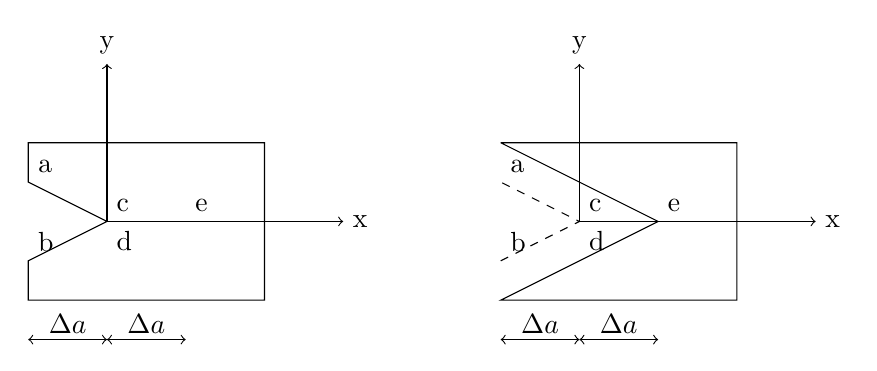
\begin{tikzpicture}[scale=2]
		\draw[<->] (0,1) node[above] {y} -- (0,0) -- (1.5,0) node[right]{x};
		\draw (0,0) node[above right] {c} -- (-0.5,0.25) node[above right] {a} -- (-0.5,0.5) -- (1,0.5) -- (1,-0.5) -- (-0.5,-0.5) -- (-0.5,-0.25) node[above right] {b} -- (0,0) node[below right] {d};
		\draw (0.5,0) node[above right] {e};
		\draw[<->] (3,1) node[above] {y} -- (3,0) node[above right] {c} node[below right] {d}-- (4.5,0) node[right]{x};
		\draw[dashed] (2.5,-0.25) node[above right] {b} -- (3,0) -- (2.5,0.25) node[above right] {a};
		\draw (2.5,0.5) -- (4,0.5) -- (4,-0.5) -- (2.5,-0.5) -- (3.5,0) node[above right] {e} -- (2.5,0.5);
		\draw[<->] (-0.5,-0.75) -- (0,-0.75);
		\draw[<->] (0,-0.75) -- (0.5,-0.75);
		\draw[<->] (2.5,-0.75) -- (3,-0.75);
		\draw[<->] (3,-0.75) -- (3.5,-0.75);
		\draw node at (-0.25,-0.65) {$\Delta a$};
		\draw node at (0.25,-0.65) {$\Delta a$};
		\draw node at (2.75,-0.65) {$\Delta a$};
		\draw node at (3.25,-0.65) {$\Delta a$};
		\end{tikzpicture}
	\end{frame}
	
	\begin{frame}{modified crack closure}
		\begin{itemize}[<+->]
			\item If we assume the mesh size is small relative to the crack length, and the distance between nodes are evenly spaced in the crack tip region, we can use the displacement at nodes $(a)$ and $(b)$ instead
			\item This requires only one simulation
			\item $\Delta a / a \le 0.05$
			\begin{equation}
			G_I = \frac{1}{2\Delta a} F_y^{(c)} \left(u_y^{(a)}-u_y^{(b)}\right)
			\end{equation}
		\end{itemize}
	\end{frame}
	
	\begin{frame}{modeling in abaqus}
		\begin{itemize}[<+->]
			\item Most of these methods will apply in some fashion to other FE software tools
			\item First draw the net shape (taking symmetry into account)
			\item In this example, I am drawing 1/4 of a middle-cracked plate
			\item Partition the edge so that you can easily separate the crack tip from the plate
			\item It is helpful to add some partitions now for meshing purposes later, a box or circle/semi-circle around the crack tip
		\end{itemize}
	\end{frame}
	
	\begin{frame}{modeling in abaqus}
		\begin{figure}
		\centering
		\includegraphics[width=0.7\linewidth]{../Figures/partition}
		\label{fig:partition}
		\end{figure}
	\end{frame}
	
	\begin{frame}{modeling in abaqus}
		\begin{figure}
		\centering
		\includegraphics[width=0.7\linewidth]{../Figures/specialty_elements}
		\label{fig:specialty_elements}
		\end{figure}
	\end{frame}
	
	\begin{frame}{modeling in abaqus}
		\begin{itemize}[<+->]
			\item If you are modeling a symmetric part, make sure to impose the appropriate symmetric boundary conditions
			\item In my case, I use XSYMM (U1 = UR2 = UR3 = 0) on the left edge
			\item On the bottom edge, I use YSYMM (U2 = UR1 = UR3 = 0) on the portion of the bottom edge which is not cracked
			\item To mesh, be sure to seed the edges, this is where partitioning comes in handy
		\end{itemize}
	\end{frame}
	
	\begin{frame}{modeling in abaqus}
		\begin{figure}
			\centering
			\includegraphics[width=0.7\linewidth]{../Figures/meshed}
			\label{fig:meshed}
		\end{figure}
	\end{frame}
	
	\begin{frame}{modeling in abaqus}
		\begin{figure}
			\centering
			\includegraphics[width=0.7\linewidth]{../Figures/result}
			\label{fig:results}
		\end{figure}
	\end{frame}
	
	\begin{frame}{modeling in abaqus}
		\begin{itemize}[<+->]
			\item To post-process results, we need the force acting on the crack tip and the displacement one node away
			\item In this case, we assume, due to symmetry, that $u_y^{(a)}-u_y^{(b)} = 2 u_Y^{(a)}$
			\item To get nodal values in ABAQUS, from the Visualization module we use Tools -> Query -> Node -> Probe Values
			\item The variable corresponding to $F_y$ in ABAQUS is RF2
			\item We also probe the nodal value of displacement one node away, $u_y$ in ABAQUS is U2
		\end{itemize}
	\end{frame}
	
	\begin{frame}{modeling in abaqus}
		\begin{itemize}[<+->]
			\item When using the direct method, we need to get values of either displacement or stress along a path
			\item In ABAQUS this is done in two steps, first Tools -> Path -> Create -> Node List
			\item Next do Tools -> XY Data -> Create -> Path
			\item Choose the path you created, the variable you need (either $u_y$ or $\sigma_{yy}$) and hit Plot
			\item Next export the data for processing in Excel (Report -> XY -> Choose file name, de-select "Append to file")
			\item You can now paste this data into Excel for processing
		\end{itemize}
	\end{frame}
	
	\begin{frame}{cohesive elements}
		\begin{itemize}[<+->]
			\item Cohesive elements are one way to model crack propagation
			\item We need to know the crack path in advance, we model the the crack growth using a traction-separation law
			\item The cohesive zone theory assumes stress can never reach infinity, the maximum allowable stress in a material is the stress required to separate atoms
			\item The stress required to separate the atoms changes as a function based on their Traction-Separation law, until the atomic bond is broken
		\end{itemize}
	\end{frame}
	
	\begin{frame}{cohesive zone}
		\begin{figure}
		\centering
		\includegraphics[width=0.7\linewidth]{../Figures/cohesive_zone}
		\label{fig:cohesive_zone}
		\end{figure}
	\end{frame}
	
	\begin{frame}{traction separation}
		\begin{figure}
		\centering
		\includegraphics[width=0.7\linewidth]{../Figures/traction_separation}
		\label{fig:traction_separation}
		\end{figure}
	\end{frame}
	
	\begin{frame}{cohesive zone uses}
		\begin{itemize}[<+->]
			\item In practice, the cohesive zone can be used to model crack growth
			\item It is most often used to model de-bonding of adhesives
			\item Also commonly used to model delamination in composites
		\end{itemize}
	\end{frame}
	
	\begin{frame}{dcb}
		\begin{figure}
		\centering
		\includegraphics[width=0.9\linewidth]{../Figures/dcb1}
		\end{figure}
	\end{frame}
	
	\begin{frame}{dcb}
		\begin{figure}
			\centering
			\includegraphics[width=0.9\linewidth]{../Figures/dcb2}
		\end{figure}
	\end{frame}

	\begin{frame}{dcb}
		\begin{figure}
			\centering
			\includegraphics[width=0.9\linewidth]{../Figures/dcb3}
		\end{figure}
	\end{frame}

	\begin{frame}{dcb}
		\begin{figure}
			\centering
			\includegraphics[width=0.9\linewidth]{../Figures/dcb4}
		\end{figure}
	\end{frame}

	\begin{frame}{dcb}
		\begin{figure}
			\centering
			\includegraphics[width=0.9\linewidth]{../Figures/dcb5}
		\end{figure}
	\end{frame}

	\begin{frame}{dcb}
		\begin{figure}
			\centering
			\includegraphics[width=0.9\linewidth]{../Figures/dcb6}
		\end{figure}
	\end{frame}

	\begin{frame}{dcb}
		\begin{figure}
			\centering
			\includegraphics[width=0.9\linewidth]{../Figures/dcb7}
		\end{figure}
	\end{frame}

	\begin{frame}{dcb}
		\begin{figure}
			\centering
			\includegraphics[width=0.9\linewidth]{../Figures/dcb8}
		\end{figure}
	\end{frame}

	\begin{frame}{dcb}
		\begin{figure}
			\centering
			\includegraphics[width=0.9\linewidth]{../Figures/dcb9}
		\end{figure}
	\end{frame}
		
	\begin{frame}{extended finite element method}
		\begin{itemize}[<+->]
			\item Traditional methods need the mesh to conform to a discontinuity (crack) to model it
			\item XFEM treats the discontinuity as an additional degree of freedom within an element
			\item A key advantage of this method is that the mesh does not need to conform to the discontinuity
			\item This is done using nodal enrichment functions, which model the singularity near the crack tip
		\end{itemize}
	\end{frame}
	
	\begin{frame}{xfem}
		\begin{figure}
		\centering
		\includegraphics[width=0.9\linewidth]{../Figures/xfem1}
		\end{figure}
	\end{frame}
	
	\begin{frame}{xfem}
		\begin{figure}
			\centering
			\includegraphics[width=0.9\linewidth]{../Figures/xfem2}
		\end{figure}
	\end{frame}
	
	\begin{frame}{xfem}
		\begin{figure}
			\centering
			\includegraphics[width=0.9\linewidth]{../Figures/xfem3}
		\end{figure}
	\end{frame}
	
	\begin{frame}{xfem}
		\begin{figure}
			\centering
			\includegraphics[width=0.9\linewidth]{../Figures/xfem4}
		\end{figure}
	\end{frame}
	
	\begin{frame}{xfem}
		\begin{figure}
			\centering
			\includegraphics[width=0.9\linewidth]{../Figures/xfem5}
		\end{figure}
	\end{frame}
	
	\begin{frame}{xfem}
		\begin{figure}
			\centering
			\includegraphics[width=0.9\linewidth]{../Figures/xfem6}
		\end{figure}
	\end{frame}
	
	\begin{frame}{xfem}
		\begin{figure}
			\centering
			\includegraphics[width=0.9\linewidth]{../Figures/xfem7}
		\end{figure}
	\end{frame}
	
	\begin{frame}{xfem}
		\begin{figure}
			\centering
			\includegraphics[width=0.9\linewidth]{../Figures/xfem9}
		\end{figure}
	\end{frame}
	
	\section{damage in composites}
	
	\begin{frame}{fatigue mechanisms in a lamina}
		\begin{itemize}[<+->]
			\item One challenge in dealing with fatigue  in composites is that there are different mechanisms
			\item For low-cycle fatigue (high loads), failure can occur directly in fibers, each successive load will cause more fibers to fail
			\item For intermediate loads, matrix cracking and crack growth can occur
			\item For low loads, crack propagation will not occur in a lamina 
			\item Composite laminae have a relatively high fatigue limit, leading many to neglect fatigue in composites
		\end{itemize}
	\end{frame}
	
	\begin{frame}{fatigue mechanisms in laminates}
		\begin{itemize}[<+->]
			\item In laminates the same mechanisms apply as in a lamina, with one additional consideration
			\item In laminates, cracks can also develop (or propagate to) the boundary between layers
			\item Delamination can then occur, while individual laminae remain intact, the strength of the structure is compromised as the layers are no longer bound together
		\end{itemize}
	\end{frame}
	
	\begin{frame}{delamination}
		\begin{itemize}[<+->]
			\item In laminate theory, the assumption is made that the shear stress $\tau_{xz}$ is zero
			\item This is a good assumption away from the edges of a part, however this stress term sharply increases near the free edge
			\item This stress term can initiate cracks between layers at the edge
			\item In this region, the assumptions of a perfectly bonded laminate no longer hold, and unexpected damage propagation can occur
		\end{itemize}
	\end{frame}
	
	\begin{frame}{impact damage}
		\begin{itemize}[<+->]
			\item In general, composites are much stronger in-plane
			\item This leads to poor impact damage behavior, as an impact can generate significant out-of-plane damage
			\item This is another challenge for composites in aircraft
		\end{itemize}
	\end{frame}
	
	\begin{frame}{other issues}
		\begin{itemize}[<+->]
			\item Analysis for fracture in composites is much more complicated than for a homogeneous material
			\item How does matrix crack interact with fibers when it approaches them?
			\item Cracks also behave differently in an anisotropic material
			\item Fiber-matrix interface can cause mixed-mode conditions even when remote load is not
			\item Ply boundaries behave differently than interior
			\item Fiber concentration is not uniform
			\item Work force is not trained in anisotropic/heterogeneous analysis
		\end{itemize}
	\end{frame}
	
	\begin{frame}{advantages}
		\begin{itemize}[<+->]
			\item Damage tolerant failure (weak fibers fail first, strong fibers remain)
			\item Material properties can be tailored to specific use cases
			\item Different composites can be designed for different use cases (high temperature ceramic-matrix composites)
			\item Can improve the damage tolerance of a material (SiC-SiC composites allows use of a brittle ceramic in many advanced aircraft)
			\item Self-healing
			\item Out-of-autoclave (on-site) repair
			\item Adhesive joining (reduce holes, fastener count)
		\end{itemize}
	\end{frame}
\end{document}
